%% div-->ps-->pdf
\documentclass[10pt]{beamer}
%%\usepackage{upgreek}
%%\usepackage{hyperref}
%% Fonts
 
\usepackage[scaled]{helvet}
\usepackage{lmodern}


\usefonttheme{serif}
\usefonttheme{professionalfonts} 
\usefonttheme{structurebold} 

 
\hypersetup{backref, pdfpagemode=FullScreen}

%% Color & Theme
\definecolor{SUblue}{RGB}{0,45,100}
\usecolortheme[RGB={0,45,100}]{structure} 
\usetheme{Boadilla} 

%% Options
 

\setbeamertemplate{navigation symbols}{}
\setbeamerfont{title}{size=\large}
\setbeamerfont{frametitle}{size=\large}
\setbeamercolor{title}{fg=white, bg= SUblue!80!white}
 

%\setbeamertemplate{background}{
\includegraphics[width=3cm]{sulogo.jpg}}


\title[Regression Density Estimation]{Flexible modeling of conditional
    distributions using smooth mixtures of asymmetric student \emph{t} densities}
\author[Feng Li]{Feng Li \\ \scriptsize{ (\emph{joint with Mattias Villani and Robert
      Kohn})}} 

\institute[\emph{Dept. of Statistics}, SU]{Department of Statistics\\ Stockholm University}
\logo{
\includegraphics[height=0.8cm]{sulogo.eps}} 
\date{September 16, 2009}
 

%%%%%%%%%%Pending%%%%%%%%%%%%%%%%%%%%%%%%%%%%%%%%%%%%%%%%%%%%%%%%%%%%%%%%%%%%%%%%%%%%%%%%%
%% ``Student t densities'' or ``Student's t densities''

%%%%%%%%%%%%%%%%%%%%%%%%%%%%%%%%%%%%%%%%%%%%%%%%%%%%%%%%%%%%%%%%%%%%%%%%%%%%%%%%%%%%%%%%%%

\begin{document}


%% Title page
\begin{frame}[plain]
\titlepage
%\ThisCenterWallPaper{sulogo.jpg}
\end{frame}   

%% Outline
\section*{Outline}
\begin{frame}  
\frametitle{Outline of the talk}
\tableofcontents
\end{frame}

\section{Mixture distributions}
\begin{frame}[shadow theme]
\frametitle{Mixture distributions} 
\begin{itemize}
\item For a given $x$, a mixture distribution $p(y|x)$ is a finite mixture
  \[
  \sum\limits_{k = 1}^K {\omega _k f_k \left( {y_i |\theta _k } \right),~i = 1,...,n.} 
  \]

\item Latent variable formulation for MCMC

  \[
  \begin{gathered}
    \Pr \left( {s_i  = k} \right) = \omega _k  \hfill \\
    y_i |\left( {s_i  = k} \right)\sim f_k \left( {y_i |\theta _i } \right) \hfill \\ 
  \end{gathered} 
  \]

\item Two-block Gibbs sampler
  
  \begin{itemize}
  \item Sample $s=(s_1,..., s_n)$ conditional on ($\theta_1,...,\theta_k$).
  \item Sample each $\theta_k$ conditional on the allocation $s$.  
  \end{itemize}

\item A smooth mixture model is a finite mixture density with weights that are smooth
  function of the covariates, e.g 

\[
\omega _k \left( x \right) = \frac{{\exp \left( {x'\gamma _k } \right)}}
{{\sum\nolimits_{r = 1}^K {\exp \left( {x'\gamma _r } \right)} }}
\]


\end{itemize}

\end{frame}

\section{ME, SMR and SAGM models} 
\begin{frame}
\frametitle{ME, SMR and SAGM models}
%\framesubtitle{}

\begin{itemize}

\item Mixture-of-Experts (ME) (Jacobs \emph{et al.} (1991))
  \begin{itemize}
    \item A mixture of regressions where the mixing probabilities are functions of
      covariates.
    \item Flexibly model the mean regression and frequently used in the machine learning literature.   
    \item The components are often linear homoscedastic regressions or even constant functions. 
    \item \textit{simple-and-many} approach.  
    \end{itemize}


%%%%%%%%%%%%%%%%%%%%%%%%%%%%%%%%%%
\item Smoothly Mixing Regression (SMR) (Geweke \& Keane (2007))
  \begin{itemize}
  \item A generalization of the ME model for regression density estimation 
  \item Fail to fit heteroscedastic data even with a very large number of components
  \end{itemize}

%%%%%%%%%%%%%%%%%%%%%%%%%%%%%%%%%%%
\item Smooth Adaptive Gaussian Mixtures (SAGM) (Villani \emph{et al.} (2008))
\begin{itemize}
\item A smooth finite mixture of Gaussian densities with the mixing probabilities.
\item The \textbf{mixing probabilities}, the \textbf{components means} and \textbf{components variances} modeled as functions of the
covariates.
\item Bayesian variable selection are in all three sets of covariates. 
\item  \textit{complex-but-few} approach --- Enough flexibility is used within the mixture
  components so that the number of  components can be kept  to a minimum. 

\end{itemize}

\end{itemize}
\end{frame}


\section{Smooth mixture of asymmetric student's {\em t} densities}   
\begin{frame}
\frametitle{Smooth mixture of asymmetric student's {\em t} densities}
\framesubtitle{The model}
\begin{itemize}
\item The split-\emph{t} density is
\[
c \cdot \kappa \left( {\mu ,\phi ,v} \right)I\left( {y \leq \mu } \right) + c \cdot \kappa \left( {\mu ,\lambda \phi ,v} \right)I\left( {y > \mu } \right),
\]
where $ \kappa \left( {\mu ,\phi ,v} \right) = \left( {\frac{v}
{{v + \frac{{\left( {y - \mu } \right)^2 }}
{{\phi ^2 }}}}} \right)^{\left( {v + 1} \right)/2} $ is the kernel of student \emph{t} density and $c$ is the normalization constant.

\item  Each of the four parameters $\mu,\phi,\lambda$ and $\nu$ are connected
to covariates as
% \begin{split}
% \mu & = \beta_{\mu0}+x_{t}'\beta_{\mu} \\
% \ln\phi & =  \beta_{\phi0}+x_{t}'\beta_{\phi} \\
% \ln\lambda & =  \beta_{\lambda0}+x_{t}'\beta_{\lambda}\\
% \ln\nu & =  \beta_{\nu0}+x_{t}'\beta_{\nu}
% \end{split}
\[
\begin{split}
  \mu  &= \beta _{\mu 0}  + x_t '\beta _\mu   \hfill \\
  \ln \phi  &= \beta _{\phi 0}  + x_t '\beta _\phi   \hfill \\
  \ln \lambda & = \beta _{\lambda 0}  + x_t '\beta _\lambda   \hfill \\
  \ln v &= \beta _{v0}  + x_t '\beta _v  \hfill \\ 
\end{split} 
\]

but any smooth link function can equally well be used in the MCMC
methodology.
\item This make it possible e.g. to have the degrees of freedom smoothly varying over
  covariate space; to capture skewness and excess kurtosis with the components.
\item \emph{Common} components if $\beta _\mu=\beta _\phi=\beta _\lambda=\beta _v$, else  \emph{separate} components. 
\end{itemize}
\end{frame}

\begin{frame}[plain]
\begin{center}
\begin{figure}
    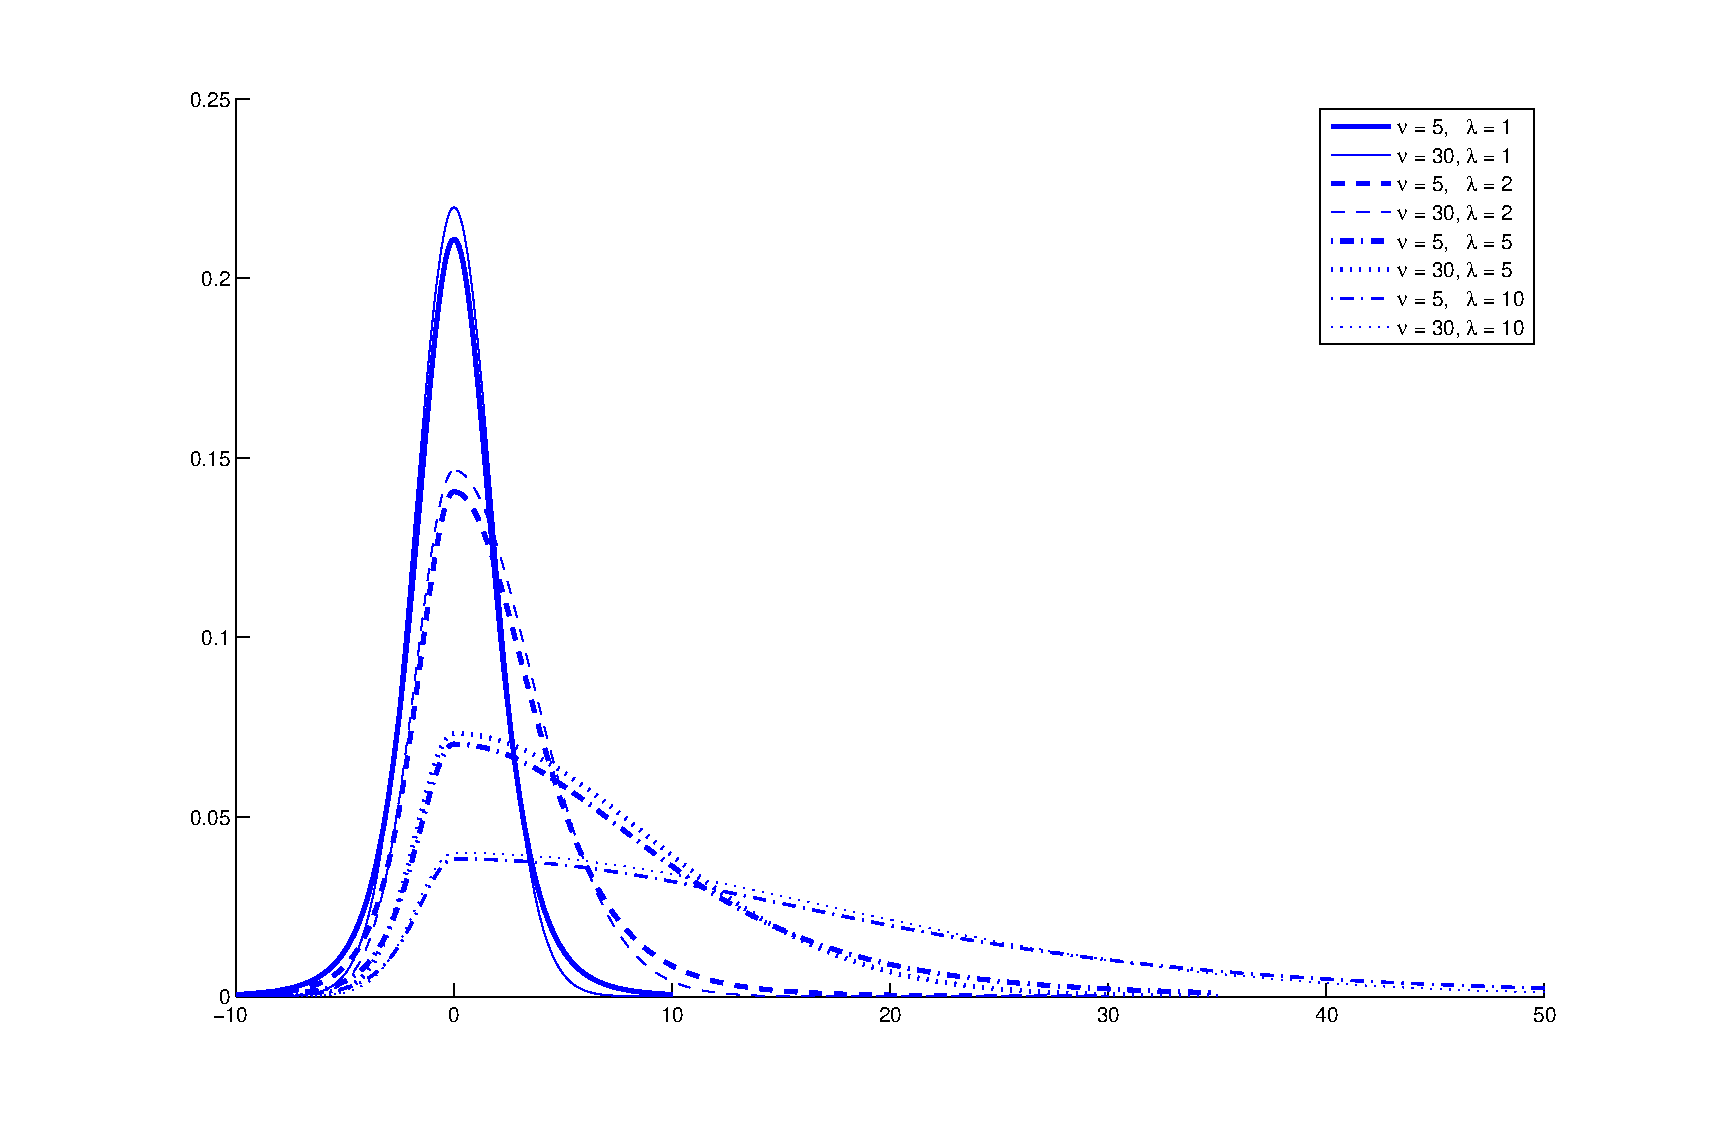
\includegraphics[height=8.4cm]{Density_Skewness.eps}
    \caption{\footnotesize{Graphical display of the split-t density with location
        parameter $\mu = 0$ and scale parameter $\lambda= 1.8$.}}\label{fg:sp500} 
  \end{figure}
\end{center}
\end{frame}


\begin{frame}
\frametitle{Smooth mixture of asymmetric student's {\em t} densities}
\framesubtitle{Discussion --- Why not over-fit?}
\begin{itemize}
\item The prior
\begin{itemize}
\item We use an easy specified prior,  $\beta|\mathcal{I} \sim N(0, \tau_{\beta}^2I)$, where $\mathcal{I}$ is the covariate
  indicators. 
\item We investigate the sensitivity of the posterior inferences and model comparison with
  respect to $\tau_{\beta}$.  
\item One can use the \emph{g}-prior $\beta \sim N(0, \tau_{\beta}^2(X'X)^{-1})$ (Zellner, 1986)
  which is less appealing in a mixture context.  
\end{itemize}
\item Variable selection (details in next page)
\begin{itemize}
\item Automatically reduce the model's complexity.
\item Investigate the importance of covariates.
\item More efficient.
\end{itemize}
\item Automatically add components to make each component simpler.  
\item Evaluating the out-of-sample log predictive density score(LPDS) -- details in
  ``model comparison'' .
\end{itemize}
\end{frame}
 

\begin{frame}
\frametitle{Smooth mixture of asymmetric student's {\em t} densities}
\framesubtitle{Inference --- Finite Newton Proposals}
\begin{itemize}
\item In a general regression model, the likelihood function is $p\left( {y|\beta } \right) = \prod\nolimits_{i = 1}^n
  {p\left( {y_i |\phi _i } \right)} $ where $k\left( {\phi _i } \right) = x_i '\beta $ (link function).
\item We need first two derivatives of $\ln p(y_i|\phi_i)$ with respect to $\phi_i$.
\item We do Bayesian variable selection within MCMC. 
\begin{itemize}
\item Set up variable selection indicator $\mathcal{I}=(I_1,...,I_n)$ where $I_i=1$
  indicates $X_i$ are in the model and $I_i=0$ means $\beta_i=0$. 
\item Sample $\beta$ and $I$ by using finite-step Newton's method. We only iterate a few
  steps($\leq$3). 
\item Dimension might change
  here. But exploits that $k(\phi_i)=x_i'\beta$ always has the same dimension (Villani \emph{et at.} 2008).
\end{itemize}

\end{itemize}
\end{frame}


\begin{frame}
\frametitle{Smooth mixture of asymmetric student's {\em t} densities}
\framesubtitle{Model comparison}
\begin{itemize}
\item Why not marginal likelihood?

  \begin{itemize}
  \item The key quantity is Bayesian model comparison is the marginal likelihood.
  \item The marginal likelihood is sensitive to the choice of prior, which is especially true when
    the prior is not very informative (Kass, 1993).  
  \end{itemize}
\item We use \emph{B}-fold cross-validation of the log predictive density score(LPDS) 

  \begin{itemize}
  \item $B^{ - 1} \sum\limits_{b = 1}^B {\ln p\left( {\tilde y_b |\tilde y_{ - b} ,x}
      \right)} $ 

  \item Compute the LPDS for ME, SMR, SAGM and our split model with different components.
  \item Compare the differences of LPDS. 
  \end{itemize}

\end{itemize}
\end{frame}




\section{Application to daily S\&P 500 returns}
\begin{frame}
\frametitle{Application to daily S\&P 500 returns}
\framesubtitle{The data}
\begin{itemize}
\item Response variable: Daily returns from S\&P 500 index.
\item Covariates
  \begin{itemize}
      \item \textbf{LastDay, LastWeek, LastMonth}, Moving average of returns from the
        previous one, five and 20 trading days respectively.
      \item \textbf{CloseAbs80, CloseAbs95}, Geometrically declining average of past
        returns $\left( {1 - \varphi } \right)\sum\nolimits_{s = 0}^\infty  {\varphi ^s
          |y_{t - 2 - s} |} $  with $\varphi$ of $.80$ and $.95$ respectively. 
      \item \textbf{CloseSqr80, CloseSqr95}, The square root of $\left( {1 - \varphi } \right)\sum\nolimits_{s = 0}^\infty  {\varphi ^s
          y_{t - 2 - s}^2} $  with $\varphi$ of $.80$ and $.95$ respectively.
      \item \textbf{MaxMin80, Maxmin95}, Information of volatility -- $\left( {1 - \varphi } \right)\sum\nolimits_{s =
          0}^\infty  {\varphi ^s \left( {\ln p_{t - 1 - s}^{(h)}  - \ln p_{t - 1 -
                s}^{(l)} } \right)} $ with $\varphi$ of $.80$ and $.95$ respectively.
  \end{itemize}

\item The models are estimated using 4646 trading days from 1990-Jan-01 to
  2008-May-29(before finical crisis). 
\item The models are evaluated out-of-sample on the 199 trading days from 2008-May-30 to
  2009-Mar-13(finical crisis period). 

\end{itemize}
\end{frame}    
\begin{frame}[plain]
%\frametitle{Application to daily S\&P 500 returns}
\begin{center}
\begin{figure}
    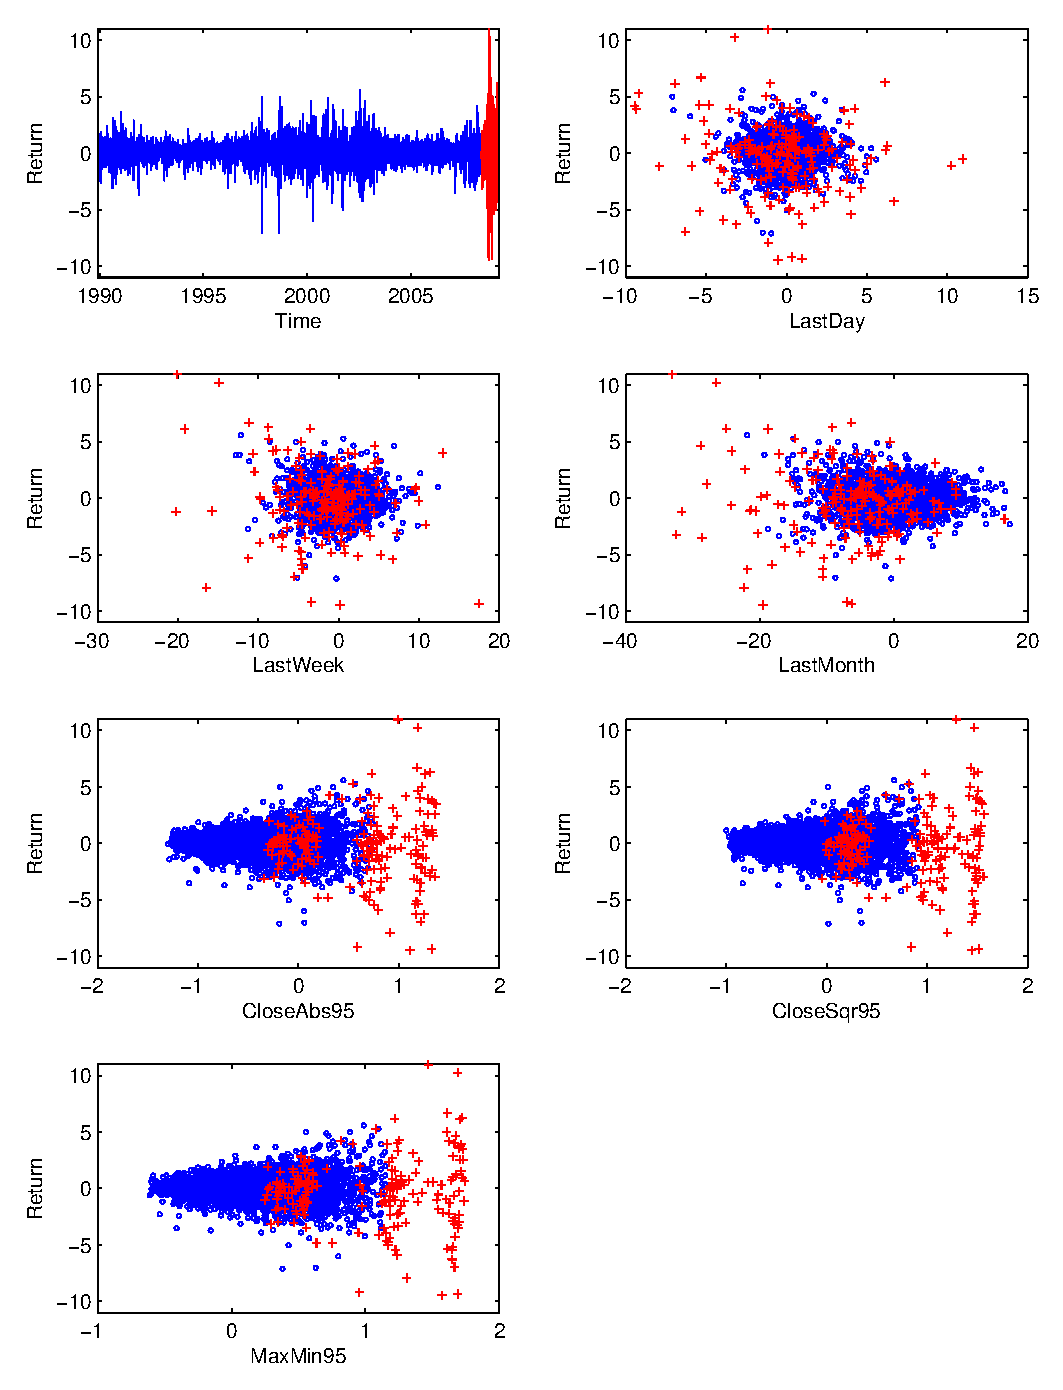
\includegraphics[height=8.4cm]{SP500Data.eps}
    \caption{\footnotesize{Time series plot of Return(up-left) and scatter plots of Return against a
        covariate(others) for S\&P500 (1990-Jan-01 -- 2009-Mar-13).}}\label{fg:sp500} 
  \end{figure}
\end{center}
\end{frame}

\begin{frame}
\frametitle{Application to daily S\&P 500 returns}
\framesubtitle{Results}
\begin{itemize}
\item A normalized residuals is defined as $\Phi^{-1}(F(y_t))$, where $F(y_t)$ is the
  cumulative predictive distribution. If the model is correct, the normalized residuals
  should be \emph{iid} $N(0,1).$  

\item The LPDS is reported for different models.
\item Posterior summary of the one-component split-t model 
\end{itemize}

\end{frame}


\begin{frame}[plain]
\begin{center}
  \begin{figure}
    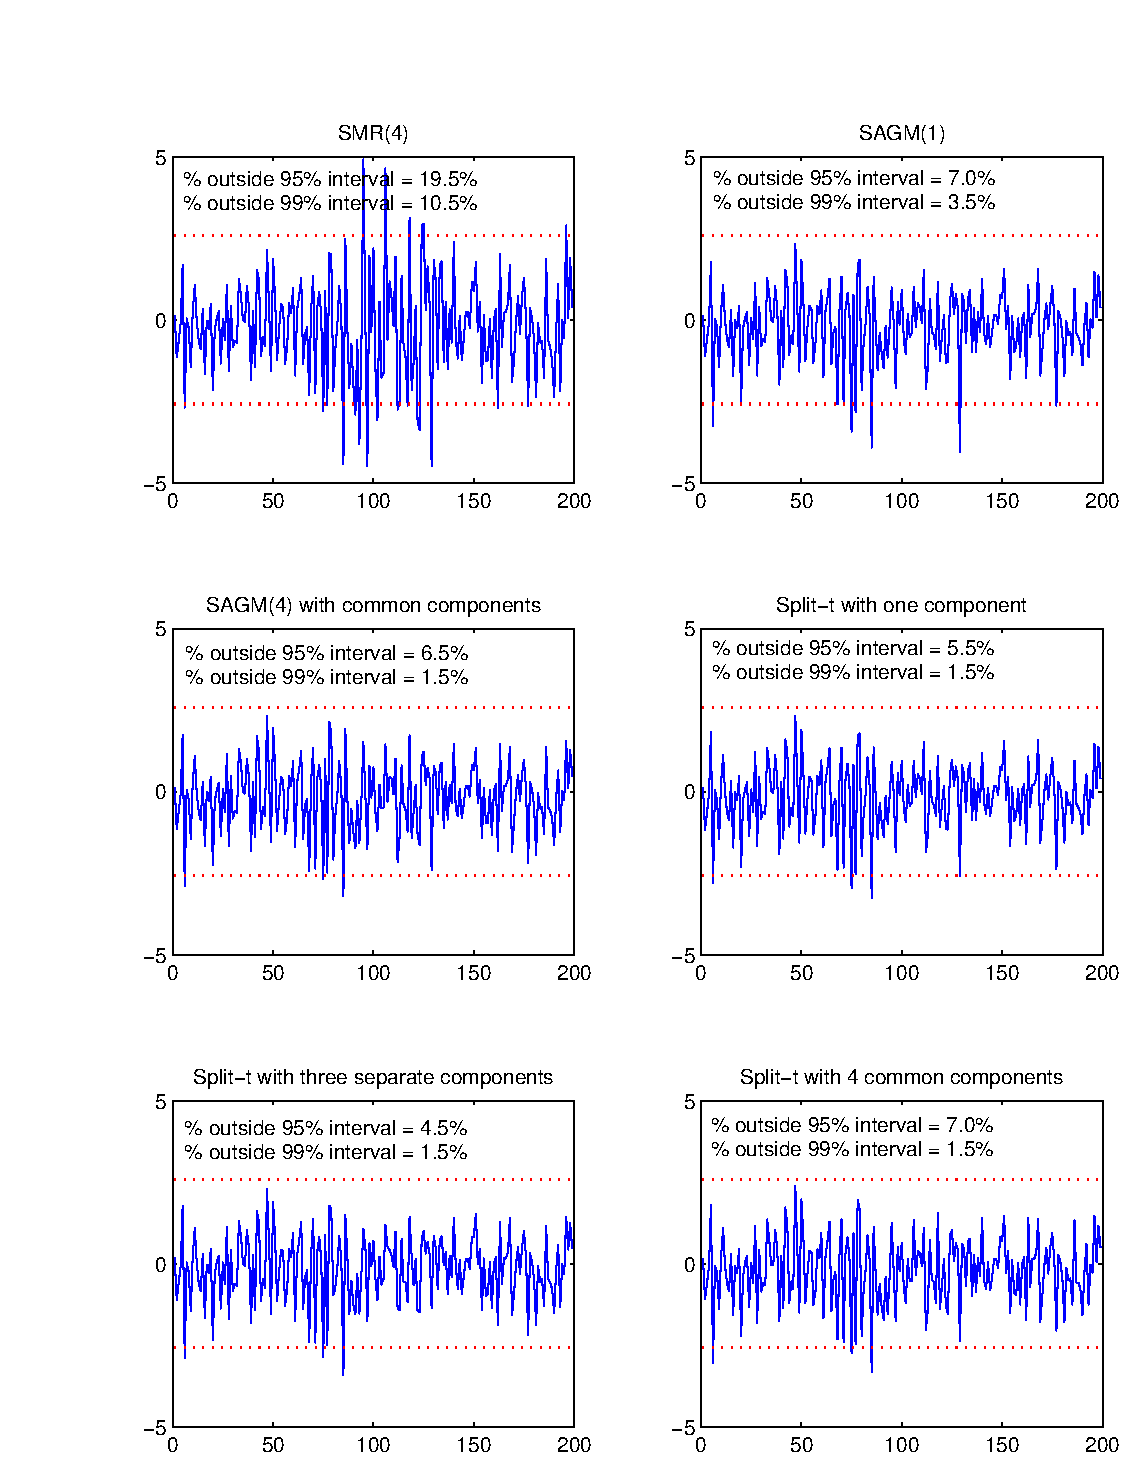
\includegraphics[height=8.4cm]{normResidPlot.eps}
  \caption{\footnotesize{The 199 normalized residuals in the evaluation sample over
time and  the 99\% probability intervals under the N(0, 1).}} 
  \end{figure}
\end{center}

\end{frame}



\begin{frame}[plain]
\footnotesize{
\begin{center}
\begin{table} 
\begin{tabular}{lccccccc}
 &  &  &  &  &  &  & \tabularnewline
\hline
\hline 
 &  &  &  &  &  &  & \tabularnewline
Model & $K=1$ & $K=2$ & $K=3$ & $K=4$ & $K=5$   & Max n.s.e.\tabularnewline
\hline
 &  &  &  &  &   & \tabularnewline
SMR & $-1044.78$ & $-638.89$ & $-505.74$ & $-487.11$ & $-489.19$   & $0.98\,(3)$\tabularnewline
+ Skew & $-540.91$ & $-525.07$ & $-513.85$ & $-506.68$ & $-506.13$  & $0.82\,(2)$\tabularnewline
+ DF & $-544.00$ & $-518.71$ & $-498.93$ & $-500.14$ & $-494.29$   & $0.89\,(1)$\tabularnewline
+ Skew + DF & $-530.86$ & $-504.63$ & $-498.03$ & $-498.83$ & $-496.87$   & $0.88\,(5)$\tabularnewline
 &  &  &  &  &    & \tabularnewline
SAGM Common & $-477.73$ & $-473.10$ & $-473.12$ & $-470.30$ & $-472.86$  & $0.26\,(2)$\tabularnewline
+ Skew & $-474.18$ & $-467.29$ & $-468.75$ & $-467.93$ & $-467.22$   & $0.35\,(4)$\tabularnewline
+ DF & $-474.74$ & $-472.92$ & $-470.51$ & $-469.40$ & $-468.87$   & $0.34\,(4)$\tabularnewline
+ Skew + DF & $\mathbf{-472.37}$ & $-468.92$ & $-469.30$ & $-466.21$ & \textbf{$\mathbf{-465.86}$}   & $0.53\,(4)$\tabularnewline
 &  &  &  &  &   & \tabularnewline
SAGM Separate &  & $-469.21$ & $-469.50$ & $-470.53$ & $-471.02$   & $0.49\,(3)$\tabularnewline
+ Skew &  & $-468.48$ & $-466.93$ & $-467.48$ & $-468.02$   & $0.58\,(4)$\tabularnewline
+ DF &  & $-469.08$ & $-469.24$ & \textbf{$\mathbf{-462.03}$} & $-467.78$   & $0.72\,(5)$\tabularnewline
+ Skew + DF &  & $\mathbf{-466.84}$ & $\mathbf{-462.56}$ & $-462.47$ & $-474.58$   & $0.74\,(5)$\tabularnewline
 &  &  &  &  &    & \tabularnewline
GARCH(1,1) & $-479.03$ &  &  &  &   & \tabularnewline
$t$-GARCH(1,1) & $-477.39$ &  &  &  &   & \tabularnewline
 &  &  &  &  &   & \tabularnewline
\hline
\hline 
 &  &  &  &  &   & \tabularnewline
\end{tabular}  

\caption{\footnotesize{Evaluating the out-of-sample log predictive density score (LPDS)}}
\label{Table: LPDS}
\end{table}
\end{center} 
}
\end{frame}



% \item Model comparison.
% \item Posterior summary of the one-component split-t model.   


\begin{frame}[plain]
\tiny{ 
\begin{table}  
\begin{centering}
\begin{tabular}{lrrrr}
 &  &  &  & \tabularnewline
\hline
\hline 
Parameters  & Mean  & Stdev  & Post.Incl.  & IF \tabularnewline
\hline 
 &  &  &  & \tabularnewline
\multicolumn{5}{c}{Location $\mu$}\tabularnewline
\hline
Const & \multicolumn{1}{r}{0.084} & \multicolumn{1}{r}{0.019} & \multicolumn{1}{r}{--} & \multicolumn{1}{r}{9.919}\tabularnewline
 &  & \multicolumn{1}{c}{} &  & \tabularnewline
\multicolumn{5}{c}{Scale $\phi$}\tabularnewline
\hline
Const & \multicolumn{1}{r}{0.402} & \multicolumn{1}{r}{0.035} & \multicolumn{1}{r}{--} & \multicolumn{1}{r}{7.125}\tabularnewline
LastDay  & \multicolumn{1}{r}{-0.190} & \multicolumn{1}{r}{0.120} & \multicolumn{1}{r}{0.036} & \multicolumn{1}{r}{0.903}\tabularnewline
\textbf{LastWeek} & \multicolumn{1}{r}{\textbf{-0.738}} & \multicolumn{1}{r}{\textbf{0.193}} & \multicolumn{1}{r}{\textbf{0.985}} & \multicolumn{1}{r}{\textbf{18.519 }}\tabularnewline
\textbf{LastMonth} & \multicolumn{1}{r}{\textbf{ -0.444}} & \multicolumn{1}{r}{\textbf{0.086}} & \multicolumn{1}{r}{\textbf{0.999}} & \multicolumn{1}{r}{\textbf{4.133}}\tabularnewline
CloseAbs95 & \multicolumn{1}{r}{0.194} & \multicolumn{1}{r}{0.233 } & \multicolumn{1}{r}{0.035 } & \multicolumn{1}{r}{1.445}\tabularnewline
CloseSqr95 & \multicolumn{1}{r}{ 0.107 } & \multicolumn{1}{r}{0.226 } & \multicolumn{1}{r}{0.023} & \multicolumn{1}{r}{2.715}\tabularnewline
\textbf{MaxMin95} & \multicolumn{1}{r}{\textbf{1.124}} & \multicolumn{1}{r}{\textbf{ 0.086 }} & \multicolumn{1}{r}{\textbf{1.000 }} & \multicolumn{1}{r}{\textbf{6.012}}\tabularnewline
CloseAbs80 & \multicolumn{1}{r}{ 0.097 } & \multicolumn{1}{r}{ 0.153 } & \multicolumn{1}{r}{0.013} & \multicolumn{1}{r}{--}\tabularnewline
CloseSqr80 & \multicolumn{1}{r}{ 0.143} & \multicolumn{1}{r}{ 0.143} & \multicolumn{1}{r}{0.021} & \multicolumn{1}{r}{--}\tabularnewline
MaxMin80 & \multicolumn{1}{r}{ -0.022 } & \multicolumn{1}{r}{ 0.200} & \multicolumn{1}{r}{0.017 } & \multicolumn{1}{r}{--}\tabularnewline
 &  &  &  & \tabularnewline
\multicolumn{5}{c}{Degrees of freedom $\nu$}\tabularnewline
\hline
Const & 2.482  & 0.238 & -- & 5.708\tabularnewline
LastDay  & 0.504 & 0.997 & 0.112 & 2.899\tabularnewline
\textbf{LastWeek} & \textbf{-2.158} & \textbf{ 0.926} & \textbf{0.638} & \textbf{5.463}\tabularnewline
LastMonth &  0.307 & 0.833  & 0.089 & 5.560\tabularnewline
CloseAbs95 &  0.718 &  1.437 & 0.229 & 3.020\tabularnewline
CloseSqr95 & 1.350 & 1.280 & 0.279 & 2.758\tabularnewline
MaxMin95 & 1.130 & 1.488 & 0.222 & 6.564\tabularnewline
CloseAbs80 &  0.035 & 1.205 & 0.101 & 2.789\tabularnewline
CloseSqr80 & 0.363 & 1.211  & 0.112 & 3.330\tabularnewline
MaxMin80 & -1.672 & 1.172 & 0.254  & 4.178 \tabularnewline
 &  &  &  & \tabularnewline
\multicolumn{5}{c}{Skewness $\lambda$}\tabularnewline
\hline
Const & \multicolumn{1}{r}{-0.104} & \multicolumn{1}{r}{0.033} & \multicolumn{1}{r}{--} & \multicolumn{1}{r}{10.423 }\tabularnewline
LastDay  & \multicolumn{1}{r}{ -0.159} & \multicolumn{1}{r}{ 0.140} & \multicolumn{1}{r}{0.027 } & \multicolumn{1}{r}{1.170 }\tabularnewline
LastWeek & \multicolumn{1}{r}{ -0.341} & \multicolumn{1}{r}{0.170 } & \multicolumn{1}{r}{0.135} & \multicolumn{1}{r}{8.909 }\tabularnewline
LastMonth & \multicolumn{1}{r}{-0.076} & \multicolumn{1}{r}{0.112} & \multicolumn{1}{r}{0.016} & \multicolumn{1}{r}{-- }\tabularnewline
CloseAbs95 & \multicolumn{1}{r}{-0.021} & \multicolumn{1}{r}{0.096} & \multicolumn{1}{r}{0.008} & \multicolumn{1}{r}{-- }\tabularnewline
CloseSqr95 & \multicolumn{1}{r}{ -0.003 } & \multicolumn{1}{r}{ 0.108} & \multicolumn{1}{r}{0.006 } & \multicolumn{1}{r}{--}\tabularnewline
MaxMin95 & \multicolumn{1}{r}{ 0.016} & \multicolumn{1}{r}{0.075} & \multicolumn{1}{r}{0.008} & \multicolumn{1}{r}{--}\tabularnewline
CloseAbs80 & \multicolumn{1}{r}{0.060} & \multicolumn{1}{r}{0.115} & \multicolumn{1}{r}{0.009 } & \multicolumn{1}{r}{--}\tabularnewline
CloseSqr80 & \multicolumn{1}{r}{0.059} & \multicolumn{1}{r}{0.111} & \multicolumn{1}{r}{ 0.010 } & \multicolumn{1}{r}{--}\tabularnewline
MaxMin80 & \multicolumn{1}{r}{0.093 } & \multicolumn{1}{r}{0.096} & \multicolumn{1}{r}{0.013 } & \multicolumn{1}{r}{--}\tabularnewline
\hline
\hline 
% &  &  &  & \tabularnewline
\end{tabular} 
\par\end{centering}
\caption{\footnotesize{Posterior summary of the one-component split-$t$ model}}
% . The posterior
% mean, standard deviation and inefficiency factors (IF) are computed
% conditional on a covariate being in the model. The IFs are not computed
% for parameters with posterior probabilities smaller than 0.02.}
\end{table}
} 
\end{frame}

\begin{frame}[plain]
%\frametitle{Smooth mixture of asymmetric student's {\em t} densities}
\begin{center}
  \begin{figure}
    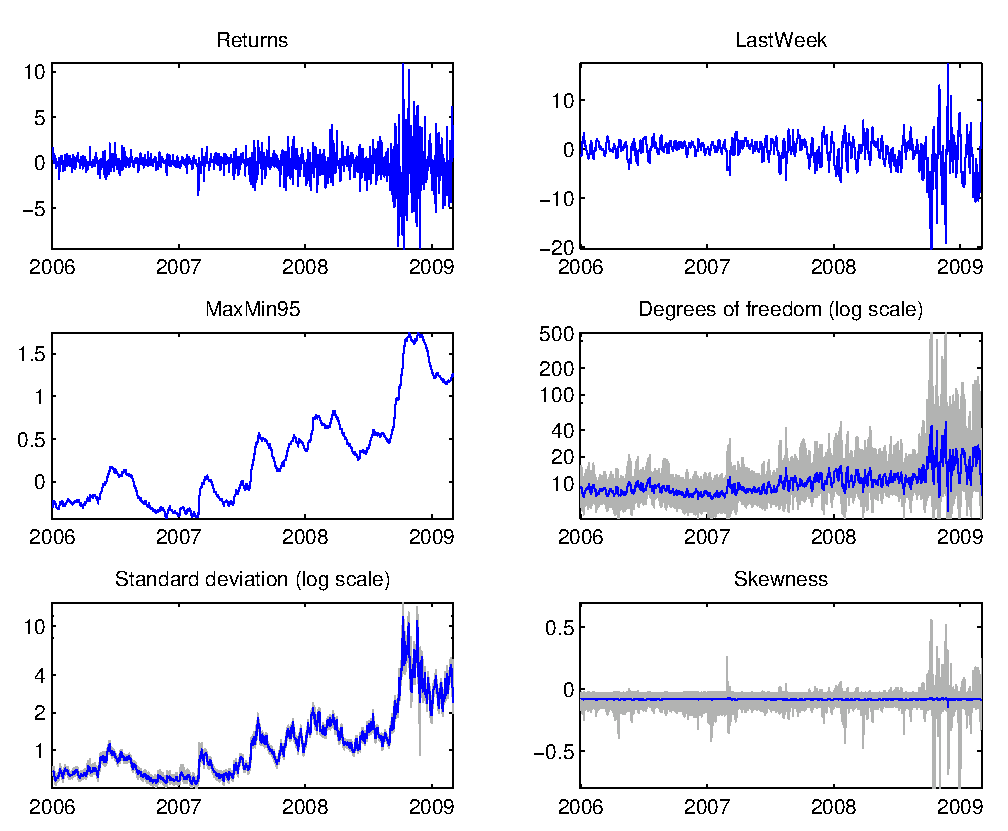
\includegraphics[height=7cm]{MomentPlotSP500.eps}
  \caption{\footnotesize{Time series plot of the posterior median and 95\% probability intervals
for some moments of the return distribution. The posterior distribution is
based on the full sample up to March 13, 2009.}}
  \end{figure}
\end{center}
\end{frame}

\begin{frame}[plain]
\begin{center}
\Huge{\color{SUblue}{Thank you!}}
\end{center}
\end{frame}

\end{document}
